\documentclass[a4paper,12pt]{article} 
\usepackage[utf8]{inputenc} % Acentos válidos sin problemas
\usepackage[spanish]{babel} % Idioma


\usepackage[backend=biber, style=alphabetic, sorting=ynt]{biblatex}
\bibliography{bibliografia.bib}
\nocite{*} % Añade todas las referencias de bib sin cita

%-----------------------------------INICIO DE PACKETES-------------------/
%-----------------------------------------------------------------------/
\usepackage{amsmath}   % Matemáticas: Comandos extras(cajas ecuaciones) |
\usepackage{amsthm}
\usepackage{amssymb}   % Matemáticas: Símbolos matemáticos              |
\usepackage{datetime}  % Agregar fechas                                 |
\usepackage{graphicx}  % Insertar Imágenes                              |
%\usepackage{biblatex} % Bibliografía                                   |
\usepackage{multicol}  % Creación de tablas                             |
\usepackage{longtable} % Tablas más largas                              |
\usepackage{xcolor}    % Permite cambiar colores del texto              |
\usepackage{tcolorbox} % Cajas de color                                 |
\usepackage{setspace}  % Usar espacios                                  |
\usepackage{fancyhdr}  % Para agregar encabezado y pie de página        |
\usepackage{lastpage}  %                                                 |
\usepackage{float}     % Flotantes                                      |
\usepackage{soul}      % "Efectos" en palabras                          |
\usepackage{hyperref}  % Para usar hipervínculos                        |
\usepackage{caption}   % Utilizar las referencias                       |
\usepackage{subcaption} % Poder usar subfiguras                         |
\usepackage{multirow}  % Nos permite modificar tablas                   |
\usepackage{array}     % Permite utilizar los valores para multicolumn  |
\usepackage{booktabs}  % Permite modificar tablas                       |
\usepackage{diagbox}   % Diagonales para las tablas                     |
\usepackage{colortbl}  % Color para tablas                              |
\usepackage{listings}  % Escribir código                               |
\usepackage{mathtools} % SIMBOLO :=                                     |
\usepackage{enumitem}  % Modificar items de Listas                      |
\usepackage{tikz}      %                                                |
\usepackage{lipsum}    % for auto generating text                       |
\usepackage{afterpage} % for "\afterpage"s                              |
\usepackage{pagecolor} % With option pagecolor={somecolor or none}|     |
\usepackage{xpatch}    % Color de lineas C & F
%\usepackage{glossaries} %                                              |
\usepackage{lastpage}    %                                              |   
\usepackage{csquotes}    %                                              |
%-----------------------------------------------------------------------\
%-----------------------------------FIN--- DE PACKETES-------------------\

\usepackage{pgfplots}     %                                             |
\pgfplotsset{compat=1.18} %           
\usepackage{etoolbox}
\usepackage{tikz,times}
\usepackage{verbatim}
\usetikzlibrary{mindmap,trees,backgrounds}
%--------------------------------/
%-------------------------------/
\usepackage[                 %   |
  headheight=15pt,  %            |
  letterpaper,  % Tipo de pag.   |
  left =1.5cm,  %  < 1 >         |
  right =1.5cm, %  < 1 >         | MARGENES DE LA PAGINA
  top =2cm,     %  < 1.5 >       |
  bottom =1.5cm %  < 1.5 >       |
]{geometry}     %                |
%-------------------------------\
%--------------------------------\

%----------------------------------------------------------------------/
%-------------------Encabezado y Pie de Pagina-----------------------/ |
%--------------------------------------------------------------------\ |
%\fancyhf{}
%\pagestyle{fancy}

\fancypagestyle{firstpage}{  
    \fancyhead[L]{}
    \fancyhead[R]{}     
    \fancyfoot[L]{}
    \fancyfoot[C]{}
    \fancyfoot[R]{\thepage\ de \pageref*{LastPage}}    
    \renewcommand{\headrulewidth}{0pt} 
    \xpretocmd\headrule{}{}{\PatchFailed}
}

\fancypagestyle{fancy}{  
    \fancyhead[L]{\textbf{Semestre: 2024-2}}
    \fancyhead[C]{}     
    \fancyhead[R]{}     

    \fancyfoot[L]{\texttt{Skynet Scribes}}
    \fancyfoot[C]{\texttt{IA}}
    \fancyfoot[R]{\thepage\ de \pageref*{LastPage}}

    \renewcommand{\headrulewidth}{1pt} 
    \xpretocmd\headrule{}{}{\PatchFailed}
    \renewcommand{\footrulewidth}{1.5pt} 
    \xpretocmd\footrule{}{}{\PatchFailed}
}

\fancypagestyle{fancyref}{  
    \fancyhead[L]{}
    \fancyhead[R]{}     
    \fancyfoot[L]{\texttt{Skynet Scribes}}
    \fancyfoot[C]{\texttt{IA}}
    \fancyfoot[R]{\thepage\ de \pageref*{LastPage}}    
    \renewcommand{\headrulewidth}{0pt} 
    \xpretocmd\headrule{}{}{\PatchFailed}
}
%--------------------------------------------------------------------\ |
%-------------------Encabezado y Pie de Pagina-----------------------/ |
%------------------------------------------------------------FIN----/


%--------------------------------------------------------------------/
%------------------- LISTA DE COLORES ------------------------------/ 
\definecolor{ProcessBlue}{RGB}{0,176,240}
\definecolor{NavyBlue}{RGB}{0,110,184}
\definecolor{Cyan}{RGB}{0,174,239}
\definecolor{MidnightBlue}{RGB}{0,103,49}
\definecolor{ForestGreen}{RGB}{0,155,85}
\definecolor{Goldenrod}{RGB}{255,223,66}
\definecolor{YellowGreen}{RGB}{152,204,112}
\definecolor{Sepia}{RGB}{103,24,0}
\definecolor{Peach}{RGB}{247,150,90}
\definecolor{CarnationPink}{RGB}{242,130,180}
\definecolor{Fuchsia}{RGB}{140,54,140}
\definecolor{WildStrawberry}{RGB}{238,41,103}
\definecolor{blueRY}{RGB}{13,164,245}

\definecolor{Grass}{RGB}{41,238,53}
\definecolor{Meadow}{RGB}{6,243,67}
\definecolor{jellyfish}{RGB}{109,14,130}
\definecolor{rubber}{RGB}{229,27,232}
\definecolor{bullet}{RGB}{225,31,90}
\definecolor{midnight}{RGB}{31,90,225}
\definecolor{sun}{RGB}{241,152,7}
\definecolor{water}{RGB}{16,229,183}

%------------------- COLORES CÓDIGO ---------------------- |
%------------------- COLORES JAVA ---------------------- |
\definecolor{backcolour}{RGB}{6,6,6} 
%\definecolor{backcolour}{RGB}{181,181,181} 
\definecolor{codeclassjava}{RGB}{246,113,59}
\definecolor{codegreen}{RGB}{17,225,48}
\definecolor{codenumizq}{RGB}{17,17,17}
\definecolor{codestringjava}{RGB}{51,240,234}
\definecolor{codesymboljava}{RGB}{255,5,0} 
\definecolor{yellowpoint}{RGB}{244,235,100} 
%------------------- COLORES JAVA ---------------------- |
%------------------- COLORES PYTHON -------------------- |
\definecolor{backcolourPY}{RGB}{6,6,6} 
%\definecolor{backcolour}{RGB}{181,181,181} 
\definecolor{codegreenPY}{RGB}{17,225,48}
\definecolor{codeclassPY}{RGB}{246,113,59}
\definecolor{codenumizq}{RGB}{17,17,17}
\definecolor{codestringPY}{RGB}{90,128,220}
\definecolor{codesymboljava}{RGB}{255,5,0} 
%------------------- COLORES PYTHON -------------------- |
%------------------- COLORES TERMINAL-------------------- |
\definecolor{backcolourTerminal}{rgb}{0.0, 0.0, 0.0} % Negro
\definecolor{codeclassTerminal}{rgb}{1.0, 1.0, 1.0} % Blanco
\definecolor{codestringTerminal}{rgb}{0.0, 0.6, 0.0} % Verde
\definecolor{codecommentTerminal}{rgb}{0.5, 0.5, 0.5} % Gris
\definecolor{codenumizqTerminal}{rgb}{0.0, 0.0, 1.0} % Azul
\definecolor{codeoptionTerminal}{rgb}{0.4, 0.4, 1.0} % Azul claro para opciones
\definecolor{yellowTerminal}{RGB}{238,200,62}
%------------------- COLORES TERMINAL-------------------- |
%------------------- COLORES CÓDIGO ---------------------- |



%------------------- LISTA DE COLORES -------------------------------\
%---------------------------------------------------------------------\

%-------------- ESTILO de Código PYTHON -----------------------------|
\lstdefinestyle{mystylepython}{
    backgroundcolor=\color{backcolourPY},
    commentstyle=\color{codecommentTerminal},
    keywordstyle=\color{blueRY},
    numberstyle=\tiny\color{codenumizq},
    stringstyle=\color{codestringPY},
    basicstyle=\footnotesize\ttfamily\color{white},
    breakatwhitespace=false,
    breaklines=true,
    captionpos=b,
    keepspaces=true,
    numbers=left,
    numbersep=5pt,
    showspaces=false,
    showstringspaces=false,
    showtabs=false,
    tabsize=2,
    escapechar=\&,
    literate=                
        {;}{{\textcolor{yellowpoint}{;}}}1
        {+}{{\textcolor{yellowpoint}{+}}}1
        {-}{{\textcolor{yellowpoint}{-}}}1
        {\{}{{\textcolor{yellowpoint}{\{}}}1
        {\}}{{\textcolor{yellowpoint}{\}}}}1
        {[}{{\textcolor{yellowpoint}{[}}}1
        {]}{{\textcolor{yellowpoint}{]}}}1
        {=}{{\textcolor{yellowpoint}{=}}}1
        {:}{{\textcolor{yellowpoint}{:}}}1
        {<}{{\textcolor{yellowpoint}{<}}}1
        {>}{{\textcolor{yellowpoint}{>}}}1
}
%-------------- ESTILO de Código PYTHON -----------------------------|
%-------------- ESTILO de Código TERMINAL ---------------------------|
\lstdefinestyle{mystyleTerminal}{
    backgroundcolor=\color{backcolourTerminal},
    commentstyle=\color{codecommentTerminal},
    keywordstyle=\color{codeclassTerminal},
    numberstyle=\tiny\color{backcolourTerminal},
    stringstyle=\color{codestringTerminal},
    basicstyle=\footnotesize\ttfamily\color{codeclassTerminal},
    breakatwhitespace=false,
    breaklines=true,
    captionpos=b,
    keepspaces=true,
    numbers=left,
    numbersep=5pt,
    showspaces=false,
    showstringspaces=false,
    showtabs=false,
    tabsize=4,    
    escapechar=\&,
    literate = 
            {--}{{\textcolor{codecommentTerminal}{--}}}2            
}
% Usar el estilo de código
\lstset{style=mystyleTerminal}
%-------------- ESTILO de Código TERMINAL ---------------------------|
\pagestyle{fancy}

\usepackage{algpseudocode}

\begin{document}%----------------------INICIO DOCUMENTO------------|
%------------------------------------------------------------------|
\begin{titlepage}
\center 
\newcommand{\HRule}{\rule{\linewidth}{0.5mm}} 

%---------------------
%	ESCUDO
%---------------------

\includegraphics[width=4.5cm]{IMA/cienciasWhite.png}

%----------------------------
%	TITULO
%----------------------------
\quad \\[0.2cm]
\textsc{\huge Facultad de Ciencias}\\[.6cm] 
\textsc{\huge Inteligencia Artificial}\\[0.5cm]

%-------------
%	TRABAJO
%-------------
\makeatletter
    \HRule \\ [0.4cm]
        { \huge \bfseries Exploradores de laberinto}\\
    \HRule \\ [0.4cm]
    
\vspace{2mm}

%----------------------------
%	Nombre del Equipo
%----------------------------
\begin{flushleft}
    \Large{Equipo:} \texttt{\Large Skynet Scribes}
\end{flushleft}
%----------------------------
%	Número de practica
%----------------------------
\begin{flushleft}
    \Large{Número de practica:} \texttt{\Large 02}\\[0.8cm]
\end{flushleft}


%-------------------
%	AUTORES
%-------------------
\begin{minipage}{0.8\textwidth}
    \begin{flushright}
        \textbf{\large{Carlos Daniel Cortés Jiménez}}\\    
        420004846        
    \end{flushright}
\end{minipage}

\vspace{5mm}

\begin{minipage}{0.4\textwidth}
        \textbf{\large{Sarah Sophía Olivares García}}\\
        318360638
\end{minipage}
\begin{minipage}{0.4\textwidth}
    \begin{flushright}
        \textbf{\large{Marco Silva Huerta}}\\
        316205326        
    \end{flushright}
\end{minipage}

\vspace{5mm}

\begin{minipage}{0.4\textwidth}
        \textbf{\large{Juan Daniel Barrera Holan}}\\    
        417079372
\end{minipage}
\begin{minipage}{0.4\textwidth}
    \begin{flushright}
        \textbf{\large{Laura Itzel Tinoco Miguel}}\\
        316020189
    \end{flushright}
\end{minipage}

\vspace{10mm}
%-------------------
%	PROFESORES
%-------------------

\begin{minipage}{0.8\textwidth}
    \begin{flushleft} \large
        Profesora: Cecilia Reyes Peña\\
        Ayudante teoría: Karem Ramos Calpulalpan \\
        Ayudante laboratorio: Tania Michelle Rubí Rojas\\                    
    \end{flushleft}
\end{minipage}

\vspace{20mm}

\begin{minipage}{0.4\textwidth}
    %---------------
    %	S E M E S T R E
    %---------------
    \textcolor{white}{Semestre}\\
    \large\textbf{Semestre 2024-2}      
\end{minipage}
\begin{minipage}{0.4\textwidth}
    %---------------
    %	F E C H A
    %---------------
    \begin{flushright}
        {\large Fecha de entrega:\\
         \textbf{28 de Febrero del 2024}}
    \end{flushright}
\end{minipage}

\makeatother

\vfill 
\end{titlepage}

\newpage
\tableofcontents

%% Investigación sobre el algoritmo
%\newpage
% ----------------------------------------------------------------------------------------\
% ---------------------------------------------------------------------------------------\
% --------------------------------------------------------------------------------------\
\section{Investigación}
% ----------------------------------------------------------------------------------------\
% ---------------------------------------------------------------------------------------\
% --------------------------------------------------------------------------------------\

% ----------------------------------------------------------------------------------------\
% ---------------------------------------------------------------------------------------\
\subsection{Fundamentos de redes bayesianas}
% ----------------------------------------------------------------------------------------\
% ---------------------------------------------------------------------------------------\


% ----------------------------------------------------------------------------------------\
% Investiga y redacta un breve resumen (máximo una cuartilla) sobre
%  qué son las redes bayesianas y para qué se utilizan.
\subsection*{Redes bayesianas}
% ----------------------------------------------------------------------------------------\
Las redes bayesianas nos permiten modelar un sistema mediante un conjunto de variables y sus respectivas relaciones de dependencia, permitiendo llevarlo a inferencia bayesiana con la que podemos estimar la probabilidad de relacionarse con variables no conocidas, con base a las conocidas. Las redes bayesianas generalmente también incluirán un conjunto de tablas de probabilidad, indicando las probabilidades para los valores verdadero o falso de las variables. 
El punto principal de las Redes Bayesianas es permitir que se realice una inferencia probabilística. Esto significa que la probabilidad de cada valor de un nodo en la red bayesiana se puede calcular cuando se conocen los valores de las otras variables.\\ 

Una red Bayesiana consta de:
\begin{itemize} 
    \item \textbf{Cualitativa} que describe las relaciones entre las distintas variables
    \item \textbf{Cuantitativa} que describe la fuerza de dichas relaciones mediante probabilidades condicionadas
\end{itemize}


Estos modelos tienen amplios usos en la clasificación, predicción, diagnostico, que brindan información sobre como se relaciones las variables llevándolos a un enfoque de causa y efecto, donde los vértices de la gráfica representan variables llamados nodos. Los nodos se representan como círculos que contienen el nombre de la variable. Las conexiones entre los nodos se nombran aristas.\\

Las redes Bayesianas se utilizan en una amplia gama de aplicaciones. Por ejemplo:

\begin{itemize}
    \item  En medicina, Las redes Bayesianas pueden ayudar a los médicos a evaluar la probabilidad de que un paciente tenga cierta enfermedad en función de los síntomas observados y los factores de riesgo.
    \item En finanzas, pueden utilizarse para evaluar riesgos y rendimientos en carteras de inversión.
    \item En reconocimiento de patrones, pueden utilizarse para clasificar imágenes o datos sensoriales.

    \item Predicción del tiempo: Pueden utilizarse para modelar la probabilidad de diferentes condiciones climáticas en función de variables como la temperatura, la presión atmosférica y la humedad.

\end{itemize}
En cada una de estas aplicaciones, las redes Bayesianas permiten modelar la incertidumbre y realizar inferencias probabilísticas sobre las variables de interés.

% ----------------------------------------------------------------------------------------\
% Explica la diferencia entre probabilidad condicional e independencia condicional, 
%  incliyendo ejemplos claros de cada uno.
\subsection{Probabilidad condicional e independencia condicional}
% ----------------------------------------------------------------------------------------\

\begin{enumerate}
    \item Probabilidad Condicional:

La probabilidad condicional se refiere a la probabilidad de que ocurra un evento dado que otro evento ya ha ocurrido. Se denota como \( P(A | B) \), que es la probabilidad de que el evento \( A \) ocurra dado que el evento \( B \) ha ocurrido. La fórmula para calcular la probabilidad condicional es:

\[ P(A | B) = \frac{P(A \cap B)}{P(B)} \]

Lo que significa que la probabilidad de \( A \) dado \( B \) es igual a la probabilidad de que ocurran ambos \( A \) y \( B \) dividida por la probabilidad de que ocurra \( B \).

Un ejemplo es: supongamos que tenemos dos eventos \( A \) y \( B \), donde \( A \) representa sacar una carta roja de una baraja estándar de 52 cartas, y \( B \) representa sacar una carta de corazones. La probabilidad de sacar una carta roja dado que hemos sacado una carta de corazones se puede calcular utilizando la fórmula de probabilidad condicional:

\[ P(A | B) = \frac{P(A \cap B)}{P(B)} \]

Donde \( P(A \cap B) \) es la probabilidad de sacar una carta roja que también sea un corazón, y \( P(B) \) es la probabilidad de sacar una carta de corazones. Si la carta roja que hemos sacado también es un corazón, entonces la probabilidad de \( A \) dado \( B \) sería \( 1/13 \), ya que hay 13 cartas de corazones en total en una baraja de 52 cartas.

\item Independencia Condicional:

Es la situación en la que dos eventos son independientes dado un tercer evento. Formalmente, dos eventos \( A \) y \( B \) son independientes condicionalmente a un evento \( C \) si la probabilidad de \( A \) dado \( B \) no cambia incluso si sabemos que \( C \) ha ocurrido. Se denota como \( A \perp\!\!\!\perp B \,|\, C \).

Por ejemplo, consideremos tres eventos \( A \), \( B \) y \( C \), donde \( A \) representa sacar una carta roja de una baraja de cartas, \( B \) representa sacar una carta de corazones y \( C \) representa sacar una carta alta (as, rey, reina o jota). Si los eventos \( A \) y \( B \) son independientes condicionalmente a \( C \), esto significa que la probabilidad de sacar una carta roja que también sea un corazón no cambia incluso si sabemos que hemos sacado una carta alta. En este caso, si \( A \) y \( B \) son independientes condicionalmente a \( C \), entonces la probabilidad de \( A \) dado \( B \) sigue siendo \( 1/13 \), incluso después de que hemos sacado una carta alta.
\end{enumerate}

% ----------------------------------------------------------------------------------------\
% Describe cómo se representa matemáticamente una red bayesiana y
%  el significado de los nodos y aristas en cada representación.
\subsection{Representación Matematica}
% ----------------------------------------------------------------------------------------\

Una red Bayesiana se define como un par \( (G, \Theta) \), donde \( G \) es un grafo dirigido acíclico (DAG) y \( \Theta \) es un conjunto de tablas de probabilidad condicional (TPC). 

El grafo \( G \) consiste en un conjunto de nodos \( V \) y un conjunto de arcos \( E \). Cada nodo representa una variable aleatoria y cada arco representa una dependencia probabilística entre las variables. Las tablas de probabilidad condicional \( \Theta \) especifican la probabilidad de cada valor posible de cada variable condicionado a los valores de sus nodos padres.

Para representar la probabilidad conjunta de todas las variables en la red, utilizamos la regla del producto:

\[
P(\text{{variables}}) = \prod_{i=1}^{n} P(X_i \,|\, \text{{padres}}(X_i))
\]

donde \( X_i \) es la variable \( i \)-ésima en la red y \( \text{{padres}}(X_i) \) son los nodos padres de \( X_i \) en el grafo.

Por ejemplo, supongamos que tenemos dos variables \( A \) y \( B \) en una red Bayesiana, donde \( B \) depende de \( A \). Podemos representar esto como:

\[
P(A, B) = P(A) \cdot P(B \,|\, A)
\]

Aquí, \( P(A) \) es la probabilidad marginal de \( A \) y \( P(B \,|\, A) \) es la probabilidad condicional de \( B \) dado \( A \). La probabilidad conjunta de \( A \) y \( B \) se calcula multiplicando la probabilidad de \( A \) por la probabilidad condicional de \( B \) dado \( A \).\\ 

% ----------------------------------------------------------------------------------------\
\subsubsection*{Modelo con nodos y aristas}
% ----------------------------------------------------------------------------------------\

Ejemplo de una red Bayesiana y los significados de los nodos y aristas:

\begin{figure}[H]
    \centering
    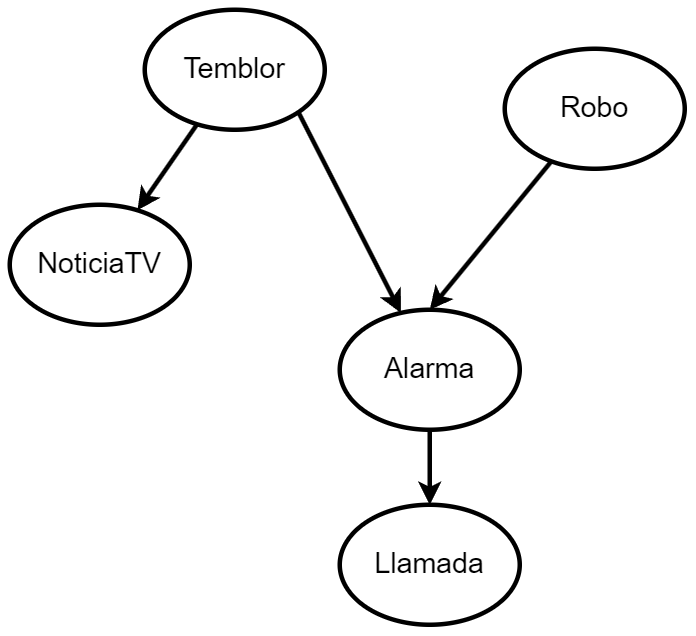
\includegraphics[width=0.35\linewidth]{IMA/RedesBayes.png} 
    \caption{Diagrama de una red Bayesiana} 
\end{figure}

Observemos estos elementos en la red Bayesiana:

\begin{itemize}
    \item Si hay un robo es más probable
    suene la alarma, lo que hace más probable que que reciba una llamada.
    
    \item Si recibo una llamada se incrementa
    la probabilidad de que haya sonado la alarma y por tanto de que me
    hayan robado
    
    \item Si oigo en la radio que ha habido un
    terremoto es más probable que éste haya ocurrido, lo que hace más
    probable que que suene la alarma.
    
    \item Si suena la alarma se incrementa la
    probabilidad de que haya ocurrido un terremoto y por tanto de que
    oiga la noticia en la television.
    
    \item Si suena la alarma y ocurre una de
    las causas (terremoto) , me creo menos que haya ocurrido el otro evento causante (robo)	
    
    \item Y viseversa, Sí suena la alarma y ocurre una de
    las causas (robo) me creo menos que haya ocurrido el otro evento causante (terremoto)
\end{itemize}

Notemos como los nodos y aristas en la red Bayesiana representan las relaciones probabilísticas entre las variables y cómo se propagan las probabilidades a través de la red. Siendo una herramienta poderosa para modelar sistemas complejos y realizar inferencias probabilísticas.
Dependiendo de nuestro enfoque de estudio, podemos utilizar las redes bayesianas para modelar sistemas complejos y realizar inferencias probabilísticas.\\ 

Elementos de una red Bayesiana:
\begin{itemize} 
    \item Nodos: Cada nodo en el grafo representa una variable aleatoria. Que representan aspectos del sistema que estamos modelando.
    \item Aristas: Las aristas representan las relaciones entre las variables. Una arista que va desde el nodo A al nodo B indica que el nodo B es dependiente del nodo A. Esto puede interpretarse como "el nodo A causa o influye en el nodo B".
\end{itemize}

Distribuciones de probabilidad condicional

\begin{itemize}
    \item Para cada nodo en la red, este tiene asociada una distribución de probabilidad condicional que describe la probabilidad de los posibles valores del nodo dado los valores de sus nodos padres.
    \item Las Distribuciones de probabilidad condicional reflejan las relaciones causales entre las variables representadas por los nodos. Por ejemplo, en una red que modela el clima y la probabilidad de lluvia, la Distribuciones de probabilidad condicional del nodo "lluvia" podría depender de los nodos "humedad"\ y "neblina".
\end{itemize}

Ventajas y limitaciones de las redes bayesianas

Las ventajas de las Redes Bayesianas son las siguientes:

\begin{enumerate} 
    \item Las Redes Bayesianas representan visualmente todas las relaciones entre las variables en el sistema con arcos de conexión.
    \item Es fácil reconocer la dependencia e independencia entre varios nodos.
    \item Las redes bayesianas pueden manejar situaciones en las que el conjunto de datos está incompleto ya que el modelo da cuenta de las dependencias entre todas las variables.
    \item Las redes bayesianas pueden mapear escenarios donde no es factible/práctico medir todas las variables debido a las limitaciones del sistema (costos, falta de suficientes sensores, etc.)
    \item Ayuda a modelar sistemas ruidosos.
    \item Se puede utilizar para cualquier modelo de sistema, desde todos los parámetros conocidos hasta ningún parámetro conocido.
\end{enumerate}

Las limitaciones de las Redes Bayesianas son las siguientes:

\begin{enumerate} 
    \item Todas diferentes caminos o ramificaciones que pueden tomar los nodos en el grafo, deben ser calculadas para calcular la probabilidad de cualquier rama.
    \item La calidad de los resultados de la red depende de la calidad de las creencias o modelos previos. Una variable es solo una parte de una red bayesiana si crees que el sistema depende de ella.
    \item El cálculo de la red es NP-duro, por lo que es muy difícil y posiblemente costoso.
    \item Los cálculos y probabilidades utilizando la regla y marginación de Bayes pueden volverse complejos.
\end{enumerate}
%-------------------------------------------

%% Desarrollo sobre el trabajo realizado
%%  para las 3 partes del problema
%\newpage
% ----------------------------------------------------------------------------------------\
% ---------------------------------------------------------------------------------------\
% --------------------------------------------------------------------------------------\
\section{Desarrollo}
% ----------------------------------------------------------------------------------------\
% ---------------------------------------------------------------------------------------\
% --------------------------------------------------------------------------------------\
% Explicación de las implementaciones, diagrama de flujo, ideas, comentarios, investigación, etc
% ----------------------------------------------------------------------------------------\
% ---------------------------------------------------------------------------------------\
\subsection{Implementación básica del Juego de la Vida}
% ----------------------------------------------------------------------------------------\
% ---------------------------------------------------------------------------------------\



% ----------------------------------------------------------------------------------------\
% ---------------------------------------------------------------------------------------\
\subsection{Introducción a los Algoritmos Genéticos}
% ----------------------------------------------------------------------------------------\
% ---------------------------------------------------------------------------------------\



% ----------------------------------------------------------------------------------------\
% ---------------------------------------------------------------------------------------\
\subsection{Implementación de Algoritmos Genéticos en el Juego de la Vida}
% ----------------------------------------------------------------------------------------\
% ---------------------------------------------------------------------------------------\
%-------------------------------------------

%% Ilustración de las pruebas realizadas
%%  y punto extra final
% ----------------------------------------------------------------------------------------\
% ---------------------------------------------------------------------------------------\
% --------------------------------------------------------------------------------------\
\section{Resultados obtenidos}
% ----------------------------------------------------------------------------------------\
% ---------------------------------------------------------------------------------------\
% --------------------------------------------------------------------------------------\
% Mostrar ejecuciones del código con capturas 
% Mostrar una comparación del código

% ----------------------------------------------------------------------------------------\
% ---------------------------------------------------------------------------------------\
\subsection{Implementación básica del Juego de la Vida}
% ----------------------------------------------------------------------------------------\
% ---------------------------------------------------------------------------------------\




% ----------------------------------------------------------------------------------------\
% ---------------------------------------------------------------------------------------\
\subsection{Implementación de Algoritmos Genéticos en el Juego de la Vida}
% ----------------------------------------------------------------------------------------\
% ---------------------------------------------------------------------------------------\




% ----------------------------------------------------------------------------------------\
% ---------------------------------------------------------------------------------------\
% --------------------------------------------------------------------------------------\
\section{Reflexión final}
% ----------------------------------------------------------------------------------------\
% ---------------------------------------------------------------------------------------\
% --------------------------------------------------------------------------------------\

% Después de las simulaciones, analizar cómo la evolución de los cromosomas afectó el 
% desarrollo del Juego de la Vida, identificando patrones o estrategias exitosas.

% Redactar un breve informe que reflexione sobre el aprendizaje obtenido, las estrategias 
% que resultaron ser más efectivas y cómo los principios de los algoritmos genéticos 
% podrían aplicarse a otros problemas de optimización o simulación.
%-------------------------------------------

% ----------------------------------------------------------------------------------------\
% ---------------------------------------------------------------------------------------\
\subsection{Modificación de Probabilidades}
% ----------------------------------------------------------------------------------------\
% ---------------------------------------------------------------------------------------\

Recordemos el modelo original, donde las redes bayesianas son las encargadas de indagar en 
la satisfacción laboral y cuenta con tres variables clave:
\begin{itemize}
    \item[] $(a)$ Horas de trabajo $(H)$: \textit{largas, moderadas o cortas}.
    \item[] $(b)$ Balance trabajo-vida $(B)$: \textit{equilibrado o no equilibrado}.
    \item[] $(c)$ Satisfacción laboral $(S)$: \textit{satisfecho, neutral e insatisfecho}.
\end{itemize}


Cuando pensé en la modificación para esta parte del trabajo pensé en un cambio que he tenido
a lo largo de la carrera ya que cuando entre, pensaba que ir a la oficina a programar sería 
algo que me hiciera muy feliz, paso el tiempo y ahora sé que el cambio que me gustaría es 
trabajar desde casas. \\ 

Trabajar desde casa no es solo para programadores o trabajos que requieran estar detras de 
una computadora, pensé en pesonas del campo, más especificamente en un pastor quien tiene que 
ver que sus ovejas no sa vayan muy lejos y si esta se va, poder encontrarla rapidamente. Es 
así como pensé en un segundo parametro para esta tarea: ayuda de inteligencia artifical (IA). \\ 

Imaginemos que el pasor esta en una zona montañosa, aunque si debe estar con sus ovejas 
la ayuda de la inteligencia artifical podría ayudar con un dron que siga a sus ovejas y si 
una sale del limite, el dron la pueda seguir y decirle al pastor donde esta. \\ 

Basicamente las dos modificaciones que se tendrán contempladas serán las de un horario más 
flexible (trabajando desde casa) y el poder contar con herramientas con inteligencia artifical
que ayuden a terminar nuestras tareas dentro del trabajo.\\ 


% ---------------------------------------------------------------------------------------\
\subsubsection*{Horas de trabajo}
% ----------------------------------------------------------------------------------------\
La flexibilidad en horarios de trabajo permitido hacerlo desde casa con ayuda de la IA nos 
da una distribución más equilibrada de las horas de trabajo ya que se pueden cumplir en 
ciertos lapsos a lo largo del día o poder terminar mucho antes y no estar un una oficina.

\begin{itemize}
    \item Valores antes: [[0.6], [0.3], [0.1]] \textit{largas, moderadas o cortas}
    \item Valores ahora: [[0.08], [0.65], [0.27]] \textit{largas, moderadas o cortas}
\end{itemize}


% ---------------------------------------------------------------------------------------\
\subsubsection*{Balance trabajo-vida}
% ----------------------------------------------------------------------------------------\
Arriba mencionamos que un horario en casa y el contar con herramientas que le permitan hacer
su trabajo más rapido podría hacer que el trabajador termine antes sus actividades lo que 
le permitira aprovechar el tiempo para hacer otras actividades en su vida.

\begin{itemize}
    \item Valores antes: [[0.4, 0.7, 0.2], [0.6, 0.3, 0.8]] \textit{equilibrado o no equilibrado}.
    \item Valores ahora: [[0.5, 0.85, 0.88], [0.5, 0.15, 0.12]] \textit{equilibrado o no equilibrado}.
\end{itemize}

% ---------------------------------------------------------------------------------------\
\subsubsection*{Satisfacción laboral}
% ----------------------------------------------------------------------------------------\

\begin{itemize}
    \item Valores antes: [[0.8, 0.05], [0.15, 0.6], [0.05, 0.35]] \textit{satisfecho, neutral e insatisfecho}.
    \item Valores ahora: [[0.88, 0.55], [0.1, 0.35], [0.02, 0.1]] \textit{satisfecho, neutral e insatisfecho}.
\end{itemize}

Para un trabajador entonces poder terminar sus activades antes y poder estar en casa para ser 
más productivo en su vida (por supuesto que es el caso optimo) encontrando balance trabajo-vida podría 
llevar a una mayor satisfacción laboral en general.

% ----------------------|
% Referencias           |
% Forma de Compilar     |
% pdflatex main.tex     |
% biber main            |
% pdflatex main.tex     |
\newpage %              |
\thispagestyle{fancyref}
\printbibliography %    |
% ----------------------|

\end{document}%----------------------F I N DOCUMENTO---------------|
%------------------------------------------------------------------|
